\section{Process' perspective}

\subsection{Team organization and interaction}
The team created a Discord channel to function as the main communication channel throughout the project. Here, the team met each Monday after the lecture to discuss what work had been completed since last week, what work had to be completed by the end of the current week, and who should do which tasks. \\
The team used Jira's Kanban Board feature\cite{jira} to gain a better overview of the various tasks. The Kanban consisted of the following columns: "To Do", "In Progress", and "Done". Hence, the team could move the tasks to the corresponding status of its progress, such that the state was visible to the rest of the team members.

\subsection{A complete description of stages and tools included in the CI/CD chains.}
\todo{Need better styling}
The CI/CD pipeline uses Github actions, Travis CI, ESLint, Sonar Cloud, and Semantic Release. Github actions is run on both the develop and main branch when a pull request or push to the repository is made. \\

ESLint is used through the github action \textit{stefanoeb/eslint-action@1.0.2} \cite{eslint-action} and is performing static code analysis by checking line indentation, unused variables, props passed to React components etc. Travis CI is integrated into the Minitwit repository and is used to run all unit tests within the Minitwit/API folder \cite{travis-ci}. Sonar Cloud is also used to perform static code analysis and checks code smells such as if code duplication exceeds 4\%. It also scans for potential security vulnerabilities \cite{sonarcloud}.

\subsubsection{Pull request}
On a pull request, the Travis CI, Sonar Cloud and the ESLint Github action are all being run. If they all pass, then the developers are allowed to perform the merge.

\subsubsection{Push}
On a push to the main or Develop branch, a \textit{Build and Push} Github action is run. The jobs builds the Frontend, API and Sim-Api Docker images and pushes them to Dockerhub. Once all three jobs have finished, a fourth job is started which ssh's into the swarm manager droplet on Digital Ocean and updates the corresponding running services in the swarm using the \textit{docker service update --image name-of-image} command. The ssh action is \textit{appleboy/ssh-action@master}\cite{ssh-action}. Below is an image taken from the Github action log showing the four jobs:

\begin{figure}[H]
    \centering
    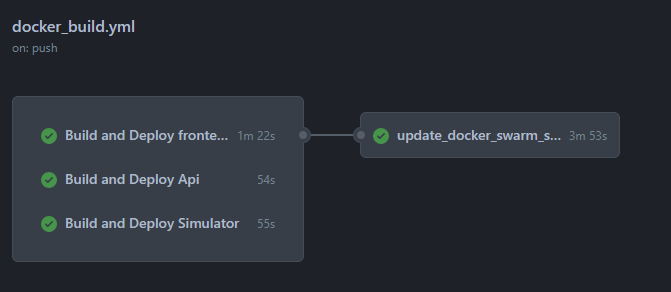
\includegraphics[width=1\linewidth]{report/images/build-and-deploy-action.png}
    \caption{Build and deploy action successfully run}
    \label{fig:build-and-deploy}
\end{figure}

Furthermore, a Github action with the name \textit{Create Release} running \textit{Semantic Release} will act on any push to the master branch with a commit name with the prefix \textit{fix}, \textit{feat} or \textit{BREAKING CHANGE}. If the commit's name fulfills the prefix, the \textit{Semantic Release} will create a new release on the main branch \cite{semantic-release}.

\subsubsection{Automating latex to pdf}
\todo{vi mangler GitHub action der konverterer Latex-rapporten til PDF}

\subsection{Organization of your repositor(ies)}
The MiniTwit application was built using a mono-repository on GitHub. The structure in the Repository consisted of a sub-folder for the API (API for the front end and the Simulator API), a sub-folder for the Frontend React Application, and a sub-folder for the report written in Latex. 

\subsection{Applied branching strategy}
The team applied the task-branching strategy\cite{branching} together with having both a Main and Develop branch. The Develop branch was initially a mirror of the Main branch and is where new functionality is developed and tested. Once a task is created on Jira and a team member has been assigned to develop it, the developer will create a branch with the task-name off of the Develop branch. Once completed and tested successfully the branch is merged into Develop. Finally, Develop was merged into Main once a week. However, this was not happening weekly in the first weeks of the project due to the team being behind schedule. 

\subsection{Applied development process and tools supporting it}
The team tried to use pair-programming in an informal manner as much as possible as opposed to assigning each member with their own task. Pair programming was preferred to allow most possible members to get hands on experience with the various DevOps themes and to enhance code quality. To facilitate pair-programming, the team utilized Discord's screen sharing functionality as well as Visual Studio Code's Live Share functionality\cite{live_share}. While screen sharing functionality is self-explanatory, the Live Share functionality provided a way for multiple developers to work on the documents simultaneously. 

\subsection{Monitoring and logging}

\subsubsection{Metrics collection}
%How do we monitor
The Prometheus container uses the 'local' network which is configured to use an overlay driver in the docker-compose.yml:

\begin{figure}[H]
    \centering
    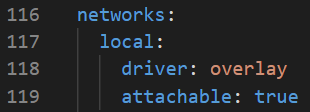
\includegraphics[width=0.4\linewidth]{report/images/LocalNetwork1.png}
    \caption{code snippet from Minitwit/docker-compose.yml}
    \label{fig:docker-compose-overlay}
\end{figure}
\noindent See appendix \ref{appendix:docker-compose} for the full compose file.\\
The services to be scraped are also running on the 'local' network.\\
This network configuration allows Prometheus to resolve the virtual ip addresses of all of the api and sim-api service replicas running in the Docker swarm. Prometheus's scraping job is configured in the Minitwit/prometheus.yml:

\begin{figure}[H]
    \centering
    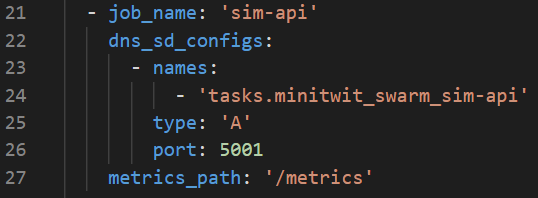
\includegraphics[width=0.66\linewidth]{report/images/LocalNetwork2.png}
    \caption{code snippet from Minitwit/prometheus.yml}
    \label{fig:prometheus-scraping}
\end{figure}
\noindent See appendix \ref{appendix:prometheus-config} for the full configuration file.\\
Here, the sim-api job scrapes all sim-api tasks/replicas by executing a DNS query to resolve their ip and then uses the specified \textit{metrics\_path} endpoint to pull the metrics.\\
As of the current setup, only the sim-api service is being scraped and not the api service.\todo{kan vi nå at fikse dette?}\\
The monitoring setup uses a pull based monitoring where Prometheus pulls the metrics from the services and Grafana pulls the metrics from Prometheus.\\

%Why is this necessary
As seen in figure \ref{fig:back-end-depencency-diagram}, both the api and sim-api uses the prom-client library to passively monitor endpoint requests and responses by "sniffing".
Prom-client is used for the whitebox monitoring as part of both of the api's middleware to monitor the total requests and responses and the individual endpoints and response codes.

%Source code:
%Using prom-client to set up the monitoring in the monitoring.js 
%Sets up middlewares in the API endpoints to monitor requests before they get to the endpoints and their responses after the endpoints.

%What precisely do we monitor
As seen in the figure \ref{fig:Monitoring1}, the Grafana dashboard display graphs for the total amount of requests and responses as well as more precise counters for the requests and responses of each endpoint in the last hour.

\begin{figure}[H]
    \centering
    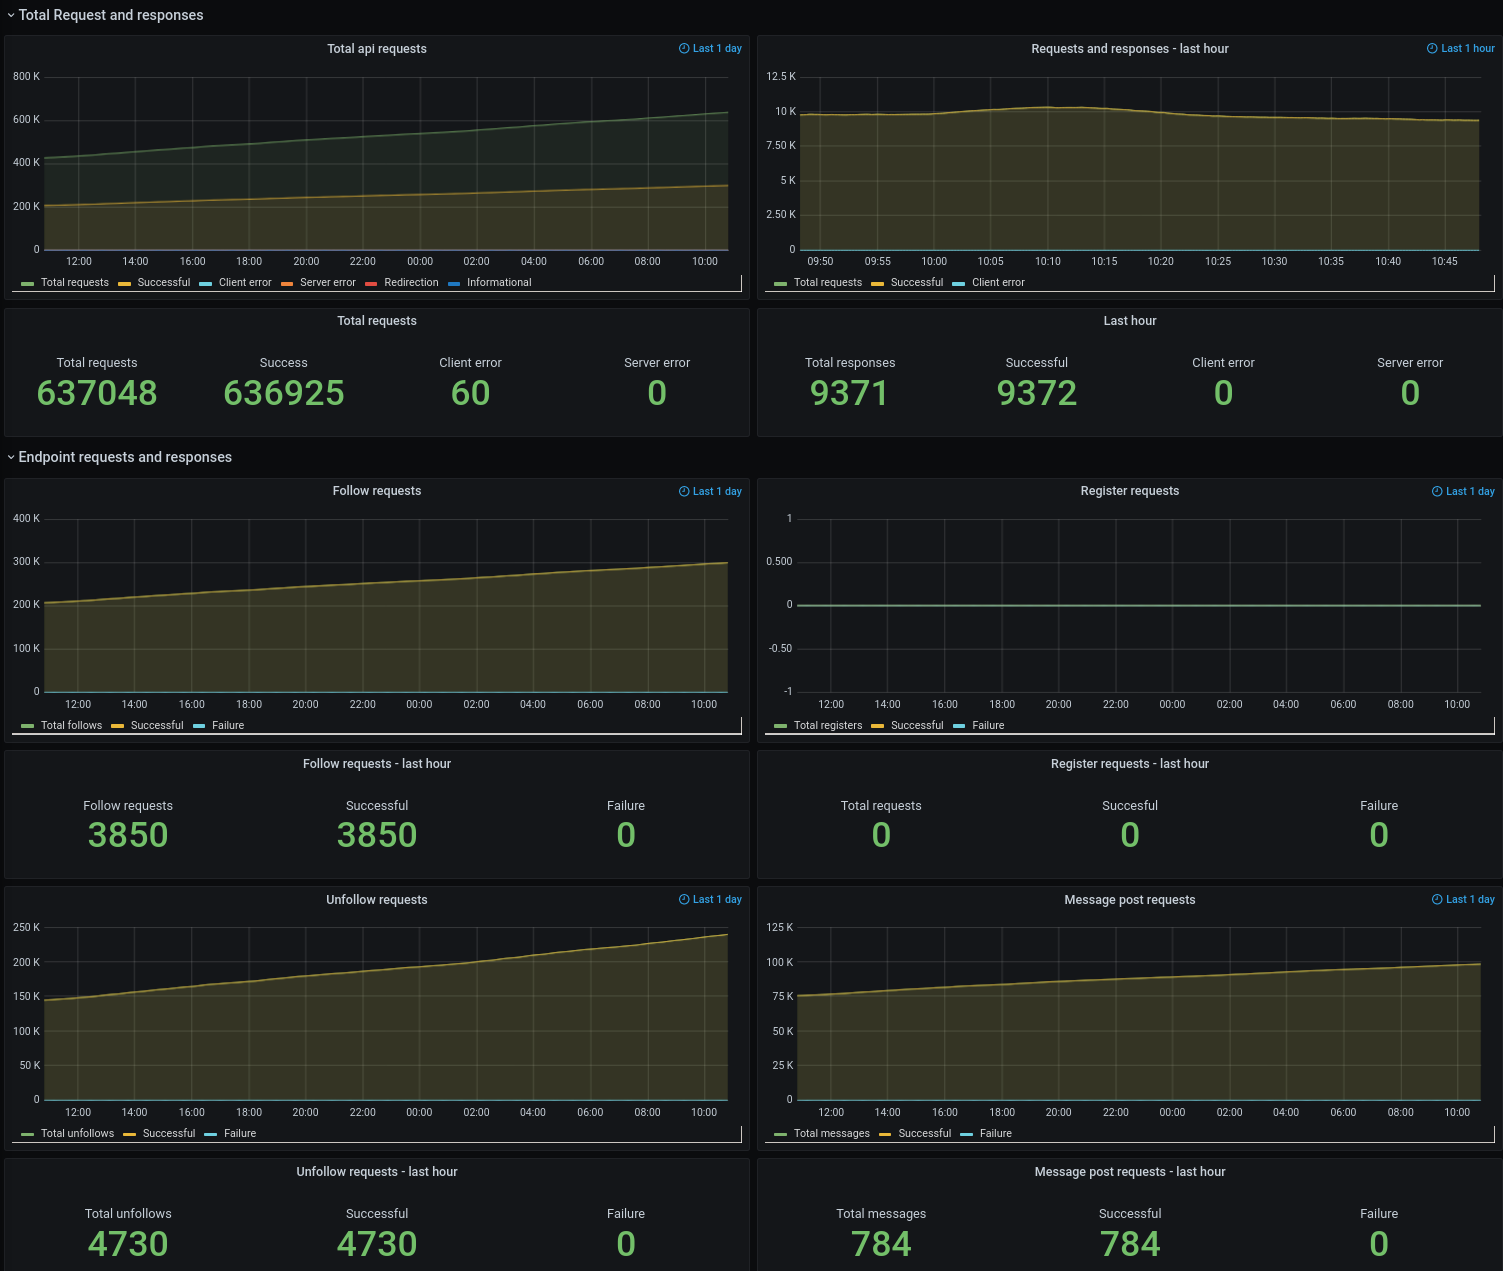
\includegraphics[width=1\textwidth]{report/images/MonitoringRequest.png}
    \caption{Request/response monitoring. \href{https://github.com/Niels-Frederik/MiniTwit/blob/main/report/images/MonitoringRequest.png}{Click here for full size image}}
    \label{fig:Monitoring1}
\end{figure}

%Reactivate vs proactive monitoring: we probably use proactive?
%Pull vs push monitoring: grafana and prometheus PULLs information!!!
%Blackbox monitoring/whitebox monitoring: We monitor existing requests and thereby checks the states and events = whitebox.
%Passive vs active monitoring: Passive monitoring - "sniffing" other requests
%Application monitoring: we monitor amount of requests 

No infrastructure monitoring



The dashboard allows for a quick overview of user activity, 
%When users are active - for analysis of user activity 
%More or less load as well as which day registers happende (in test simulation)
%quick and easy overview of which endpoints fails and how much
%Endpoints responses... Like do users or the server cause errors in specific endpoints
%Allowed us to easily see how missing users from downtime cause usererrors in endpoints....
%Maybe even downtime



\todo{Se om vi kan lave application monitoring og/eller infrastructure monitoring: response time kunne være fedt}
%Snak om at vi intet infrastructure har, men hvordan vi kunne have gjort det 

%Future optimizations...
%API isn't really monitored... only simapi

%Response time
%Do not implement unless we get more time
%write about how we would have implemented it as well as why it would be really nice to have

%The state of the Docker Swarm - container overview.


\subsubsection{Log collection and aggregation}
The system uses a Loki/Promtail/Grafana stack for logging. A loki driver is installed on both the nodes in the docker swarm service with the following command:

\begin{verbatim}
    docker plugin install grafana/loki-docker-driver:latest
    --alias loki --grant-all-permissions
\end{verbatim}

Furthermore, the \textit{/etc/docker/daemon.json} file on both nodes is modified, which allows for all docker containers to redirect their logs to the Loki endpoint via the loki driver.

\begin{verbatim}
    {
    "debug" : true,
    "log-driver": "loki",
    "log-opts": {
        "loki-url": "http://161.35.214.217/loki/api/v1/push"
    }
}
\end{verbatim}

This allows us to aggregate logs from all nodes in the docker swarm stack, which is sent to the Grafana dashboard for querying and visualization. Lastly, a Promtail container is deployed to load locally stored logs into Grafana.\\

\noindent
This stack is chosen for many different reasons:
\begin{itemize}
    \item Requires significantly less memory compared to ELK/EFK stack
    \item Utilizing Grafana for visualization, which is already used by Prometheus
    \item Easy setup and integration with docker swarm
\end{itemize}

Furthermore, the collection of logs have utilized the Winston library in order to provide an easier way to maintain how logs are stored and formatted.\cite{winston} As an example, the following so-called CustomLogFormat has been created:
\begin{verbatim}
    const customLogFormat = printf(({message, level, timestamp}) => {
        return `${timestamp} ${level}: ${message}`
    });
    
    const customLogger = createLogger({
        format: combine(timestamp(), customLogFormat),
        transports: [new transports.Console()],
    });
\end{verbatim}
This provides a log format to be used which shows the time-stamp of the log, the so-called "log level", and the log message. Hence, the logs get a common syntax, and if a change is needed in the syntax it happens at a single place.
\\\\
\todo{Færdiggør nedenstående (hvem end der startede det)}
\noindent
For the dashboard we chose to visualize 

\noindent
Currently no log rotation is implemented
%logging diagram
%Why we chose it (already grafana dashboard for monitoring, low memory usage, easy compatibility with docker swarm)
%Console log (writing to std.out, not worrying about storage)
%Loki container
%Screenshot of logs
%What things do we log from the source code
%No log rotation (modifying daemon.json)
%docker plugin install grafana/loki-docker-driver:latest --alias loki --grant-all-permissions

\subsubsection{Acting}

\subsection{Brief results of the security assessment}
\todo{Færdiggør NMAP (hvem end der startede det)}
Running NMAP showed the following open ports and services:

None of these have any exploitable weaknesses. 

\subsection{Applied strategy for scaling and load balancing}
As already mentioned, the system is hosted in Docker swarm mode with two nodes running on their own droplets in the network. The docker swarm scales horizontally, as more worker nodes running on their own physical machine can join the swarm if the swarm were to be scaled. \\
\\
With swarm comes load balancing out of the box. The ingress network exposes the services on the swarm via the routing mesh. The load balancer decides which of the running instances of the requested service the request should end up at\cite{docker-ingress}. This is seen in figure \ref{fig:arcitechture-overview} where an incoming request to the load balancer on the \textit{production-worker} droplet can be redirected to a container running within the \textit{Minitwit} component of the \textit{minitwit-webserver} droplet.

\subsubsection{Updating the swarm}
The swarm is configured to use rolling updates with \textit{--update-order} set to \textit{start-first}. For each service, an updated version is instantiated and monitored for 5 seconds before it is decided to be running successfully. Once running, the old instance of the service is shut down. This rolling update strategy is run for each service for each replica. See appendix \ref{appendix:docker-compose} for the full docker-compose.yml.\\
The start-first approach was chosen to guarantee that at least the desired amount of replicas are always run during updates.